% source: https://tex.stackexchange.com/a/229678
\begin{figure}[ht]
    \centering
    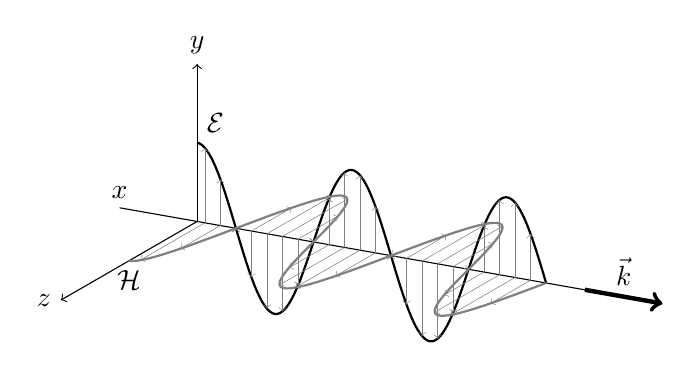
\begin{tikzpicture}[x={(-10:1cm)},y={(90:1cm)},z={(210:1cm)}]
        % Axes
        \draw (-1,0,0) node[above] {$x$} -- (5,0,0);
        \draw[->] (0,0,0) -- (0,2,0) node[above] {$y$};
        \draw[->] (0,0,0) -- (0,0,2) node[left] {$z$};
        % Propagation
        \draw[->,ultra thick] (5,0,0) -- node[above] {$\vec k$} (6,0,0);
        % Waves
        \draw[thick] plot[domain=0:4.5,samples=200] (\x,{cos(deg(pi*\x))},0);
        \draw[gray,thick] plot[domain=0:4.5,samples=200] (\x,0,{cos(deg(pi*\x))});
        % Arrows
        \foreach \x in {0.1,0.3,...,4.4} {
          \draw[->,help lines] (\x,0,0) -- (\x,{cos(deg(pi*\x))},0);
          \draw[->,help lines] (\x,0,0) -- (\x,0,{cos(deg(pi*\x))});
        }
        % Labels
        \node[above right] at (0,1,0) {$\mathcal{E}$};
        \node[below] at (0,0,1) {$\mathcal{H}$};
    \end{tikzpicture}

    \caption{Visual representation of a propagating plane wave in classical electrodynamics with $\vec k$ being the wave vector dictating the direction in which the wave propagates and is perpendicular to the wave-front \cite{Brekhovskikh1980Waves}.}
    \label{fig:em_waves}
\end{figure}
